%\documentclass[11pt]{article}
%\usepackage{framed, color}
%\usepackage{textpos}
%\usepackage{natbib}
%\usepackage{geometry}
%\usepackage[hidelinks]{hyperref}
%\usepackage{textcomp}
%\usepackage{graphicx}
%\usepackage{fancybox}
%\usepackage{setspace}
%\hypersetup{colorlinks=false, urlcolor=blue, citecolor=black}
%\usepackage{soul}
%\usepackage{geometry}
%\usepackage{fancyhdr}
%\usepackage{wrapfig}
%\usepackage{mdframed}
%\usepackage{fontspec}
%
%\renewcommand\refname{Bibliography and References Cited}
%\newgeometry{top=.5in, bottom=.5in, left=.5in, right=.5in}
%\setmainfont{Arial}
%\linespread{1.2}
%\urlstyle{same}
%\setlength{\parindent}{1cm}
%
%\begin{document}


\noindent \textbf{APPROACH}


To better understand the physiologic response to dehydration resistance, a series of experiments that will allow us to understand how differences in temperature, relative humidity, and water availability affect the desert-adapted rodent \textit{Peromyscus eremicus} will be conducted. These experiments are fundamentally a series of environmental manipulations, described in \hyperlink{Figure 1}{Figure 1}. The experimental design is fully factorial, meaning that the focal experimental parameter (e.g. water availability) will be tested in the context of the full range of other conditions (e.g. humidity, temperature). \emph{Environmental parameters are chosen to match the most extreme (hottest and driest) conditions faced by wild animals in nature}, while cool/moist conditions effectively represent a less challenging control environment. Animals are exposed to each experimental condition for 14 days. Animal care is standardized between experiments and includes measures to reduce the water content of food and bedding materials. Both of these will be dried in a standard desiccation oven to less than 10\% water/volume. Forty individuals per treatment will be included - power analyses suggest this sample size will allow for detection of statistical support for patterns with small to medium effect sizes. Together, this design will make it possible to tease-apart the physiologic and genomic response to the various conditions. \\

\vspace{2mm}

\begin{mdframed}
 \begin{center}
  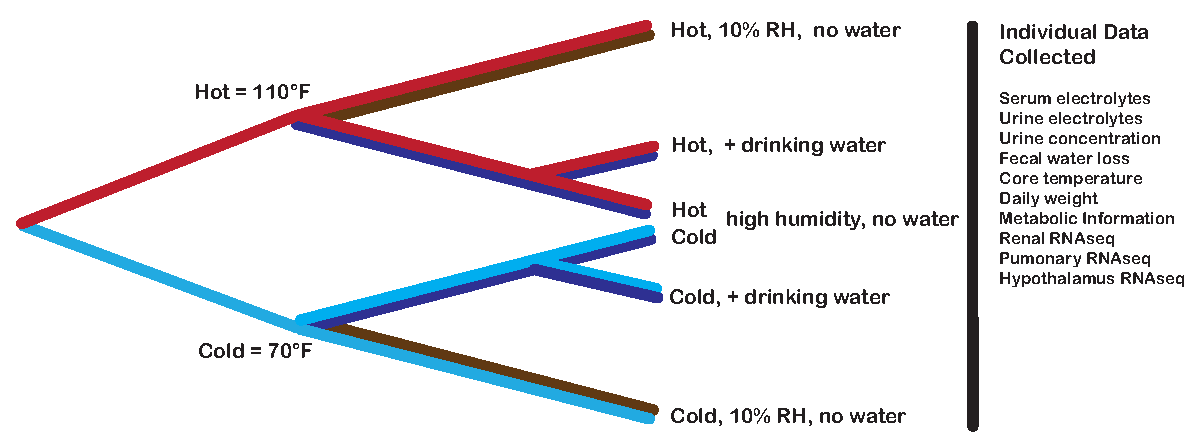
\includegraphics[width=1\textwidth]{exp_design_fig.eps}
 \end{center} 

\noindent \small{Figure 1: Animals are relegated into either hot or cold treatments. Within treatments (n=40 per treatment), animals are exposed to two weeks of varying levels of aridity, from simulated rainfall where water is available \textit{ad libitum}, to dry, where no water is available. RH=Relative Humidity}

\end{mdframed}

\vspace{3mm}

\noindent \textbf{Specific Aim 1:} \ul{Determine the physiologic response to drinking-water deprivation, extreme temperature, and humidity in the desert-adapted rodent \textit{P. eremicus}}. It is hypothesized that, as a result of unique mechanisms related to solute and water balance, average serum electrolyte concentrations will remain relatively constant throughout various experimental manipulations, but the variance in measured levels between individuals will increase in the most extreme conditions. These differences will be echoed in differences in urine electrolytes and concentration. Predictions regarding other parameters are detailed in Table 1. \\

Background: The human body consist of 60\% water \citep{Jequier:2009cz}. Far from a static reservoir, proper physiologic function requires water for countless processes including nutrient transport \citep{Haussinger:1996wl}, signal transduction, pH balance, thermal regulation \citep{Montain:1999ux} and the removal of metabolic waste. To accomplish these functions, approximately 2 liters of fluid are used daily - these fluids are lost mainly via the gastrointestinal and genitourinary systems, and by evaporative loss, which is accelerated greatly in extremes of heat and aridity \citep{Cheuvront:2010eg}. These losses must be matched by intake \citep{Jequier:2009cz}, mainly in the form of oral fluid intake. Though the body possesses limited reserves, when loss exceeds intake over even a short period of time, dehydration and in extreme cases, death can occur. Humans and most other animals are exquisitely sensitive to dehydration, and possess limited compensatory mechanisms. In contrast, desert rodents survive in extreme environmental conditions, often without fluid intake. 

Previous work in the MacManes lab has demonstrated that \peer\ is remarkable in it's drinking habits, with \textit{ad lib} water intake lower than other desert-adapted rodents (Figure 2). This suggests that Understanding the mechanisms underlying this remarkable phenotype requires we understand the physiology that \begin{wrapfigure}{r}[0pt]{.5\textwidth}
	\begin{mdframed}
 	\begin{center}} 
  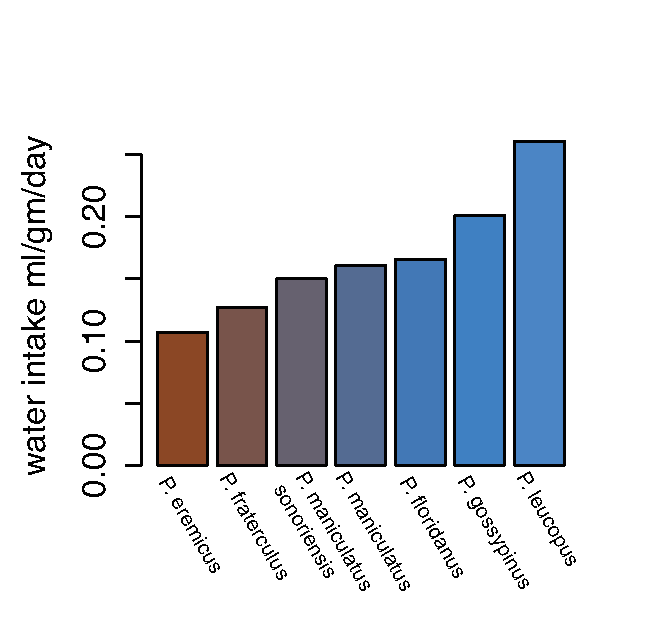
\includegraphics[width=1\textwidth]{species_water_intake.eps}
 	\end{center}} 
\noindent \small{Figure 2: When supplied with water \textit{ad lib}, individual \peer\ consume very little water relative to other \textit{Peromyscus} species, even those that are desert adapted (\textit{P. fraterculus, P. maniculatus sonoriensis}.)
	\end{mdframed}
\end{wrapfigure}
\noindent accompanies it. The work described here aims to characterize the physiology of dehydration resistance in desert adapted rodents. \\


While the prolonged absence of drinking water is invariably fatal for humans and many other animals, one potentially mitigating effect may be the acquisition of water (or limitation of loss) via the pulmonary vasculature, which is known to be variably permeable to water \citep{Berger:2011ks,Goralski:2010eo}. While pulmonary water acquisition has not been quantified in humans or in mammalian models, the pulmonary vasculature is ideally positioned to retain water from inspired air. Following this, relative humidity -  the amount of extractable water present in respired air may be important to overall hydration status. The design described above incorporates two different levels of humidity to begin to disentangle the effects of drinking water from water acquisition via the pulmonary system. \\
  

Although water stress is obviously important to the survival of desert rodents - a phenotype which is relevant to human health and wellness, extreme temperatures represent another way in which physiological processes may be challenged. While desert animals may thrive in extreme heat, humans cannot. The physiological response is characterized in model organisms, but not in other animals adapted to these conditions. Genes like the heat-shock proteins are protective in humans, but no record of their activity on desert rodents is known. \\

Research Plan:To accomplish this aim, physiologic data from animals held with and without drinking water will be gathered, factorial with respect to the other conditions (e.g. temperature and humidity). The specific experiments described in \hypertarget{Figure 1}{Figure 1} will allow us to tease apart the effects of water deprivation from other parameters. Though the data we propose to collect is described above, in brief, we plan to collect blood and urine electrolytes, urine osmolality, fecal water and electrolyte content, as well as renal parameters such as GFR (glomerular filtration rate). We will collect data on fluid intake, animal weight and temperature, as well as a battery of metabolic parameters such as oxygen and carbon dioxide production. The specific predictions regarding several of these parameters are described in Table 1.  \\

In the context of limited water intake, how animals achieve electrolyte balance is unknown. Electrolytes are both easy to assay and are critical to physiological well being. Indeed, proper electrolyte balance is fundamental to all other physiological processes like neuronal signal transduction and muscle (including cardiac) contractility. Here, serum electrolytes will be measured using the VetScan VS2 critical care panel which includes ALT, BUN, Cl, CRE, GLU, K, Na, bicarbonate ion in a 100uL sample volume. \\

In addition to assaying electrolytes themselves, measures of urine electrolytes and specific gravity will be collected, as the urinary system represents that major pathway through which these chemicals are lost. These parameters will be measured using an Atago UG-$\alpha$ urine refractometer and tests of urine osmolarity conducted at the IDEXX reference lab. Lastly, animals will be weighed to the nearest 0.1gm every other day, including the day of sacrifice. Body temperature will be assayed with weighing using a digital thermometer and probe designed by World Precision Instruments (Sarasota, FL). In connection with this, feces will be collected and water content will be measured using standard methods. \\

Key metabolic parameters such as \ul{carbon dioxide production} and \ul{oxygen consumption} that may influence water consumption will be collected. In addition, the \ul{change in relative humidity} within the metabolic chamber will be assayed, which will allow us to understand the rate of pulmonary water loss (or gain). These tests will be measured during a twenty four hour period at the end of the experimental manipulation, just prior to euthanasia, using a metabolic chamber (Sable Inc.) modified for use in the desert chamber. Together, these data will represent a uniquely rich characterization of the physiological state of a desert rodent held in captivity but more importantly, exposed to conditions typical of the natural environment. \\

Lastly, I will collect information regarding renal blood flow (including regional measurements) via renal ultrasound using the ViewSonic Vevo 3100 Imaging Platform. Of note, all procedures involving vertebrate animals conform to the guidelines provided in \citep{Sikes:2011dz} and have been approved by the University of New Hampshire Animal Care and Use Committee. \\


The statistical treatment of the data will include a linear regression (either linear or non-linear) to establish the relationships between the data. Many of these analyses will be conducted with non-parametric tests, as data 

\begin{wrapfigure}{r}[0pt]{.8\textwidth}
\hypertarget{Table 1}{}
\vspace{-5mm}
\begin{mdframed}
  \begin{center}
    \includegraphics[width=1\textwidth]{Aim1-table.eps}
  \end{center}
  \noindent{\small{Table 1: Predicted response given specific experimental manipulations. The number of arrows indicate the predicted relative magnitude of the response.}}
\end{mdframed}
\end{wrapfigure}

\noindent are often non-normally distributed nor independent. One of the most interesting comparisons will be to understand the relationship between serum sodium and urine sodium, urine concentration, fecal water content, and changes in body weight. Ultimately (e.g. Aim 2) these data will be linked with patterns of gene expression, methylation, and isoform use to gain a synthetic understanding of dehydration resistance. \\




% \begin{center}
%  \includegraphics[width=.5\textwidth]{Aim1-table.eps}
% \end{center} 
%
%\noindent \small{Table 1: Say something about predictions here.}
%
%\vspace{4mm}


Preliminary data: The electrolyte profile of 2 individuals housed at 70F, 50\% RH, water \textit{ad lib} and two individuals housed in identical conditions except that drinking water was withheld has been characterized. Despite being housed in typical laboratory conditions, these animals have remarkably unusual electrolyte panel. For instance, mean serum sodium is 152 mmol/L, chloride 105 mmol/L, potassium in an un-hemolyzed sample is unusually high at 8.1 mmol/L, while Creatinine is low, with a mean measurement of 0.25mg/dL. mean blood urea nitrogen (BUN) is 47mg/dL. In contrast, animals without \textit{ad lib} water were obviously dehydrated, with a mean serum sodium of \textgreater 170 mmol/L and chloride 126 mmol/L. Interesting severe dehydration was not complicated by renal impairment as evidenced by a mean serum creatinine of 0.3 mg/dL and BUN of 59 mg/dL. Animals lost a remarkable amount of weight, on average 28\% of total body weight. Despite this decline in weight and electrolyte derangement, animals were active as per usual. \textbf{These results are shockingly distinct from human response to dehydration, and warrant further study.}  \\  


\noindent \textbf{Aim 2:} \ul{To characterize the genomic response (differential gene expression, patterns of methylation or isoform use) to extreme water restriction and heat.} {We will understand the genetic response to extreme heat and aridity via a series of Illumina bisulfite, Illumina mRNA sequencing, and PacBio mRNA sequencing experiments, and will link these patterns to individual physiologic state as defined in Aim 1.} We hypothesize that genes responsible for water and solute transport will be particularly active in the most extreme conditions in renal and pulmonary tissues, while genes involved in the activation of the hypothalamic-neurohypophysial system will be differentially regulated in the hypothalamus.\\

Background: Broadly speaking, genes underlie the vast majority of observable phenotypes. Whether this relationship is mediated by patterns of expression (e.g. \cite{Teets:2012gt}), which itself may be mediated by differences in methylation \citep{Brenet:2011dq}, or by use of alternative splice isoforms \citep{Yukutake:2010ia}, linking genotype to phenotype is extremely difficult. In addition to these mechanisms, function (=phenotype) may be determined by post-translational modifications like phosphorylation of specific sites \citep{Anonymous:2009gb}. The identification of these mechanisms is important, not only because in doing so we gain a deeper understanding of evolution, but also because these molecular mechanisms may be later used as targets for drug development or other therapeutic intervention. With regards to resistance to dehydration, the development of novel therapies is critical, as millions of people die yearly as a consequence. \\

In model organisms, dehydration precipitates a physiological response that is largely driven by the neuroendocrine system. Very much simplified, the cascade begins with the stimulation of osmoreceptors \citep{Arsenijevic:1985bi}, which in turn stimulates neurons located in the paraventricular and supraoptic nuclei of the hypothalamus to release anti-diuretic hormone (ADH) \citep{Zingg:1986vb}. ADH then binds to vasopressin-responsive receptors located in the renal medulla, resulting in aquaporin movement to the surface of the collecting duct \citep{Nielsen:1995uq} which encourages water re-uptake. In addition to the aquaporins, the renin-angiotensin-aldosterone system \citep{Gubler:2010bh}, natriuretic peptides \citep{Totsune:1994kf}, the SLC and mTOR families \citep{Ortells:2012go}, and potentially other yet to be discovered pathways are important to water balance. Far from canonical, each stage in these cascades is dynamic and therefore pathways revealed in \textit{Mus} and humans may not be equivalent to pathways in uniquely adapted desert animals, particularly given radically different phenotypes.\\

The genomic processes related to dehydration resistance in desert animals has yet to be characterized. The few studies of genetics that have been conducted have focused on the role of expression of single members of the aquaporin gene family (but see \cite{Bartolo:2007hy}), which are large membrane-bound proteins that are critically involved in renal water transport \citep{Kwon:2009bv,Verkman:2002ww,Brown:1995vo,Nielsen:1995cb}. These studies have shown that changes in Aquaporin (AQP) protein abundance and expression may be related to water availability \citep{Boselt:2009fb, Gallardo:2005fm,Bozinovic:2003eg}. In addition to changes in expression, another study showed that the AQP4 pathway was completely lost in the desert rodent \textit{Dipodomys merriami merriami} \citep{Huang:2001ti}. Despite these studies, we have a limited understanding of the genomics of renal water and solute regulation in desert animals. While AQPs are functionally important, water and solute balance is extraordinarily complex, and therefore single-gene studies are necessarily limited in their purview. A more complete understanding of this phenotype and its mechanistic underpinnings will require a sophisticated genome-level approach, which will be the outcome of the proposed research. In contrast to the limited amount known about patterns of renal gene expression, much less is known about gene expression in other tissues, and absolutely nothing about differential methylation or isoform use, even though we know that these complexities are mechanistically important to this specific function \citep{Yukutake:2010ia,Silberstein:2004ex}. \\

Research Plan: The analysis of the genome wide patterns of response to dehydration will be conducted using the same individuals for which we collected physiology data. To accomplish this goal, RNAseq libraries for each individual and tissue (n=240 animals * 3 tissues (renal, lung, hypothalamus)) will be constructed and on HiSeq 2500. We aim to generate approximately 20 million 125nt paired-end sequences per sample, which corresponds to 30 high-output HiSeq lanes using 24-way multiplexing. \\ 

RNAseq reads derived from kidney, lung, and hypothalamus will be mapped to the existing annotated draft genome, which was sequenced using startup funds. This phase of the project will be accomplished using the short read aligner BWA \citep{Li:2013wn} and best practices previously established \citep{MacManes:2014io}. Differential expression will be evaluated via the Cufflinks package \citep{Trapnell:2012kp}, while evidence for coordinated changes in large numbers of genes will be detected using the software wcgna \citep{Langfelder:2008bd}. The MacManes lab has demonstrated expertise in this area. \\

Accurate isoform reconstruction is notoriously difficult using high-throughput short read sequence data such as that produced by Illumina HiSeq platform \citep{Pyrkosz:2013tm,Hiller:2009be}, despite the advent of longer read lengths and newer analytical techniques \citep{LeGault:2013gw,Jiang:2009bw}. In projects like this, where differential isoform use may be critical to phenotype, a different approach may be warranted. For instance, the sequencing technology available from Pacific Biosystems (PacBio) is suggested to provide a resolution to the isoform reconstruction problems \citep{Au:2013hp}, specifically because it involves a long-read single molecule sequencing strategy \citep{Eid:2009kva}.  To identify patterns of differential isoform use, we will sequence poly-A selected mRNA samples using PacBio technology available to us via one of our regional GEBRI partners at the University of Delaware. Reads will be error corrected using the program LSC \citep{Au:2012iq}, and isoforms will be identified using methods contained in \cite{Au:2013hp}. Because PacBio throughput is relatively low, which may limit the precision with which quantitation can be achieved, we will explore alternative ways to accurately estimate isoform specific expression. One previously unexplored approach involves estimating expression in the program eXpress \citep{Roberts:2012dh} using only those reads that map uniquely and unambiguously to a specific isoform. Because this approach is uncharacterized, it will be validated using a set of isoform specific PCR primers that will allow us to estimate isoform-specific expression using qPCR.  \\ 

Lastly, aside from differences in expression of isoform use, patterns of methylation could be important in the development of extreme osmoregulation - indeed, methylation has been shown to be important to many other complex phenotypes including behavior \citep{Lyko:2010dr}, metabolism \citep{Foret:2012jf}, and physiologic stress (including heat stress) response \citep{Sonna:2002dc}. To understand patterns of methylation, a large bisulfite sequence dataset will be generated, which will contain information from every individual included in the mRNAseq experiments, described above. This dataset will allow for the understanding of another layer of genomic complexity not typically available to researchers conducting RNAseq experiments in isolation. Importantly, in addition to enhancing our understanding of the mechanisms underlying dehydration tolerance, phenotypes related to differential methylation may be prime therapeutic targets.    \\


%\begin{wrapfigure}{l}[0pt]{0.6\textwidth}
%\hypertarget{Table 1}{}
%\vspace{-5mm}
%\begin{mdframed}
%  \begin{center}
%    \includegraphics[width=1\textwidth]{Aim1-table.eps}
%  \end{center}
%  \noindent{\small{Table 1: Say something about predictions here.}}
%\end{mdframed}
%\end{wrapfigure}


Preliminary Data: To date, the lab has generated a RNAseq dataset that consists of approximately 30M 150nt SE Illumina reads from the same 2 animals housed in the 'cold/simulated rain' treatment group from which physiology data was collected. We have generated \textit{de novo} transcriptome assemblies as well as mapped to the reference genome. Though the scope of the analyses is preliminary, the results are interesting. 99.7\% of the RNAseq reads map to the genome, with over 73\% mapping concordantly. This suggests that the content of the draft genome is compete and genic contiguity is high. We have recovered many of the aquaporin genes, as well as many other critical genes including vasopressin and its receptor, Renin, Angiotensin, Angiotensin Converting Enzyme, as well as the genes that code for the natriuretic peptides. We have estimated expression for all transcripts.  Interestingly, within the aquaporin genes, Aquaporins 1 and 2 had the highest expression, while expression of Aquaporin 5, 9, 10 and 12 were undetectable, though they are present in the genomic reference. \\

Expected Outcome: Upon completion of Aim 1, we will have a synthetic understanding of the physiologic and genomics patterns associated with extreme osmoregulation. These data will allow us to generate a list of genes, genomic regions, isoforms, and methylation states putatively linked to the phenotype of interest. This list is critical, and will form the basis for our first R01 submission, which will propose the development of a system where manipulation of specific genes is possible (e.g. the CRISPR/CAS9 transgenic system), thus moving the work from correlation to causation. This grant will be developed and submitted during the second year of the COBRE tenure. In addition to this, the completion of Aim 1 will allow us to become more proficient in the collection and bioinformatic analysis of physiology data. Lastly, part of Aim1b involved the development of a novel pipeline for the identification of differential isoform use using PacBio RNA sequence data. This skill will be useful to the investigator's broader scientific goals, as well as to the broader scientific community.    \\

Regarding dissemination, the work will be published in open access journals, after rapid release using preprint servers. We envision several papers that are a direct result of this work, include papers describing the physiological and metabolic response to water deprivation as well as their genomic responses. In addition, we aim to publish a more methods-oriented paper surrounding the study of isoform using PacBio data. Aside from peer-reviewed publication, results will be disseminated via social media, the PI's blog, and at the annual meeting of the Society for the Study of Evolution. \\       




\noindent \textbf{Aim 3:} \ul{Given the transition from the obligate intake of fluids as infants, to it’s complete absence later in life, the ontogeny of physiologic water conservation will be elucidated.} \\

Background: Given that desert adapted mice, capable of surviving without water are as neonates dependent on liquid intake, {the study of the ontogeny of physiologic water conservation is extremely interesting and relevant to the current work.} The study of gene expression in renal, pulmonary and hypothalamus tissue types along the transition from the intrauterine environment through birth in the context of differences in oral fluid intake is remarkably novel and will yield unique insights into physiologic water conservation. Although several studies have assayed renal gene expression in neonates, these studies have typically been limited to a small number of genes in a specific context (e.g. hypertension \citep{Sampson:2012hb,Shanmugam:1996ed}). \\

In addition to the transition from lactation-dependence through weaning, an even more fundamental transition happens at birth, which is accompanied by substantial changes in renal physiology. In utero, the large volumes of dilute urine are typically produced \citep{Wintour:1997ts} while post-birth, relatively small volumes of concentrated urine are typical. While this trend appears to be canonical in well-characterized mammal models, whether the fetuses of water-stressed desert-adapted mice follow this trend is unknown, and may be extremely revealing in the context of dehydration resistance. The proposed work aims to use a genome wide approach to characterize these transitions in desert-adapted rodents. This work will provide novel insights into fundamental biological processes, bearing hard upon dehydration resistance, a phenotype which could, if translated to biomedical intervention, save millions of lives annually.  \\  


Research Plan: This phenomenon will be explored using fetal and neonatal mice whose mothers are exposed to treatments and an abbreviated set of methods listed in Aim 1. Many of the physiological measurements  (e.g. blood and urine analyses) will be impossible to collect in very young animals secondary to sample volume requirements, though a full battery of genomic tests will be possible. To evaluate the ontogeny, five fetal and neonatal mice will be culled per treatment at four different time-points (immediately prior to birth, 2 hours after birth, mid-lactation (approximately 10 days after birth), 1 day after weaning). These time-points have been chosen as together they will allow us to assay the breadth of developmental stages.  We hypothesize that patterns of gene expression, methylation, and isoform use will resemble those common in conditions where water is available \textit{ad lib}, though the novelty of this aspect of the study limits firm predictions. \\

Expected Outcome: Upon completion of Aim 3, we will have a synthetic understanding of the genomics patterns associated with the ontogeny of extreme osmoregulation. These data, together with the data associated with Aim 1 will allow us to generate a list of genes, genomic regions, isoforms, and methylation states putatively linked to the phenotype of interest. This list is critical, and will form the basis for the next R01 submission, which will propose the development of a system where manipulation of specific genes is possible (e.g. the CRISPR/CAS9 transgenic system), thus moving the work from correlation to causation. 

\vspace{3mm}
\textbf{Table 2: Timeline}
\hypertarget{Table 2}{}
\begin{center}
\begin{tabular}{l|c c r}

\textsc{Activity} & \textsc{FY2015} & \textsc{FY2016} & \textsc{FY2017} \\
\hline \\
\textsc{Recruit PDF, grad students, undergraduates} & X & & \\
\textsc{Increase Colony Size \& ID animals for experiments } & X & & \\
\textsc{Conduct Physiology Experiments -- AIM 1} & X & & \\
\textsc{Collect \& Analyze expression data -- AIM 2} & X & & \\
\textsc{Analyze Bisulfite and PacBio data -- AIM 2} & & X & \\
\textsc{} & &  &   \\
\textsc{Animal breeding in prep for Aim 2} & & X &  \\
\textsc{Collect \& Analyze genomic data -- AIM 3} & & X & X \\
\textsc{} & &  &   \\
\textsc{Write papers \& submit} & & X & X \\
\textsc{Present results at international conference} & & X & X \\
\textsc{Prepare R01 \& and resubmit as needed} & & X & X \\
\textsc{Train Undergrad, Grad students, \& PDF} & X & X & X \\
\textsc{Disseminate info} & X & X & X \\

\end{tabular}
\end{center}
\vspace{5mm}



%\newpage
%\setcounter{page}{1}
%%\thispagestyle{empty}
%\singlespacing
%\bibliographystyle{model2-names-edit.bst}
%
%\bibliography{formatted.bib}
%
%
%
%\end{document}
